Metatext blabla.
*Hur många testade vi på?

\section{Effectiveness}

\begin{figure}[p]
  \centering
  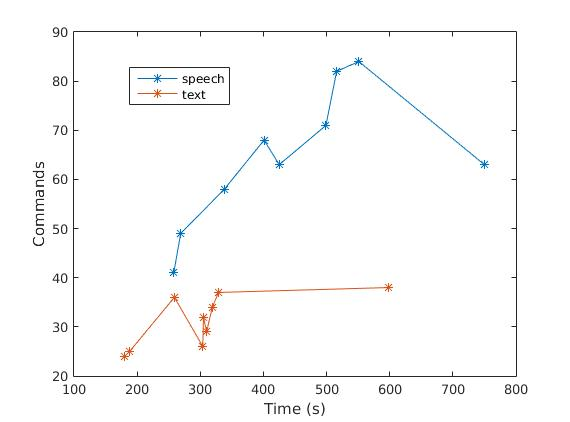
\includegraphics[width=0.8\textwidth]{images/time_cmd.jpg} %width=0.8\textwidth scales the image down to 80 percent of the text-width. Keeps the ratio.
  \caption{Bladiblala}\label{time_cmd}
\end{figure}

\subsection{Timescale} %Add standardavvikelse
Table \ref{avg_time} declares the average time in seconds it took for the users to complete each version of the game. The data shows that it takes 38\% more time to complete the speech version when compared to the text version.

\subsection{Commands} %Add standardavvikelse
Table \ref{avg_cmd} declares the average amount of commands used before completing the game. The data shows that it takes almost double (99.67\%) the amount of commands to complete the speech version when compared to the text version. This can also be seen in figure \ref{ideal_cmd}, where the average amount of commands used in each version of the game are compared to the ideal number of commands for each version. The ideal takes in consideration a realistic first playthrough of the game, where the player does not ``magically know'' what items are in each room. The ideal number of commands therefore include commands such as ``look around the room'' and ``search <item>'' to reveal a certain other item needed to complete the game. In figure \ref{ideal_cmd} it is also shown that the ideal number of commands are pretty much the same for both versions of the game, making the difference in average number of commands even more significant.

\begin{figure}[h!]
  \centering
  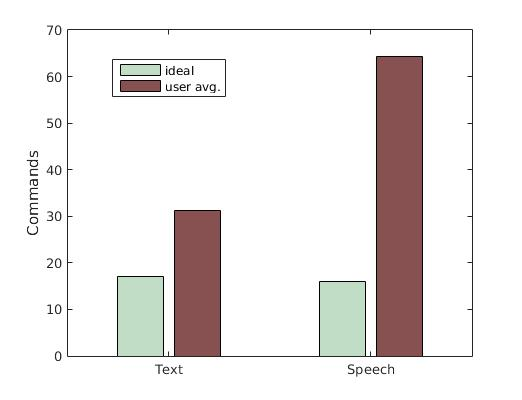
\includegraphics[width=0.8\textwidth]{images/ideal_cmd.jpg}
  \caption{Bladiblala}\label{ideal_cmd}
\end{figure}

\begin{table}[h!]
  \centering
  \begin{tabular}{ccc}
    \toprule
    Speech &   & Text\\
    \midrule
    64.33 &   & 31.22\\
    \bottomrule
  \end{tabular}
  \caption{Average Number of Commands}\label{avg_cmd} % OMG LOOK HERE!!!
\end{table}

Figure \ref{avg_time} shows the number of commands used over time. As you would expect, the speech version follows the logic of ``the longer time played the more commands used''. However, this is not the case for the text version, where the time played seems irrelevant to the amount of commands used.

\begin{table}[h!]
  \centering
  \begin{tabular}{ccc}
    \toprule
    Speech &   & Text\\
    \midrule
    445.22 &   & 310.22\\
    \bottomrule
  \end{tabular}
  \caption{Average Time}\label{avg_time}
\end{table}

\section{Ease of Use}
Bajskorv

\subsection{English Confidence}

\begin{figure}[p]
  \centering
  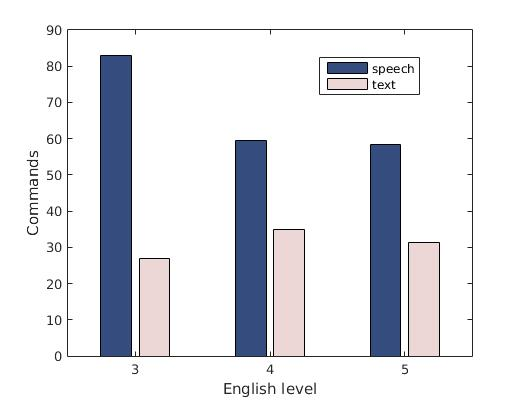
\includegraphics[width=0.8\textwidth]{images/english_cmd.jpg}
  \caption{Bladiblala}\label{eng_cmd}
\end{figure}

\begin{figure}[p]
  \centering
  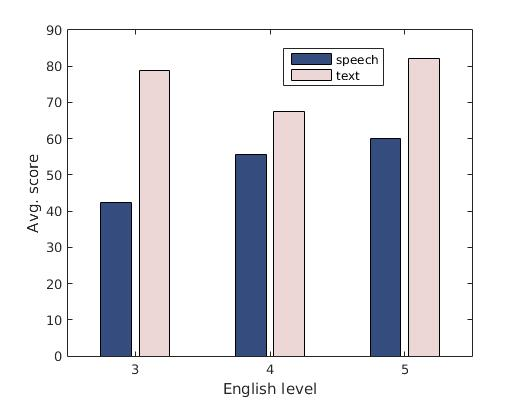
\includegraphics[width=0.8\textwidth]{images/english_score.jpg}
  \caption{Bladiblala}\label{eng_score}
\end{figure}

\begin{figure}[p]
  \centering
  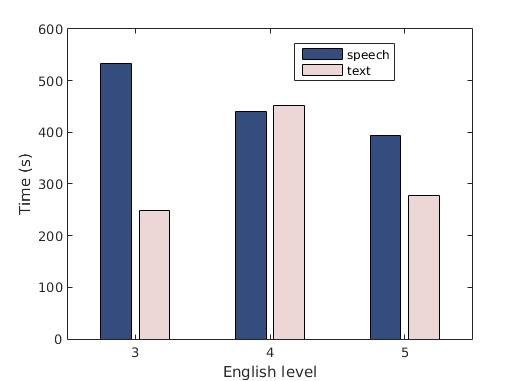
\includegraphics[width=0.8\textwidth]{images/english_time.jpg}
  \caption{Bladiblala}\label{eng_time}
\end{figure}

%\subsection{User Former Experience}

\section{Satisfaction (SUS)}

\begin{figure}[p]
  \centering
  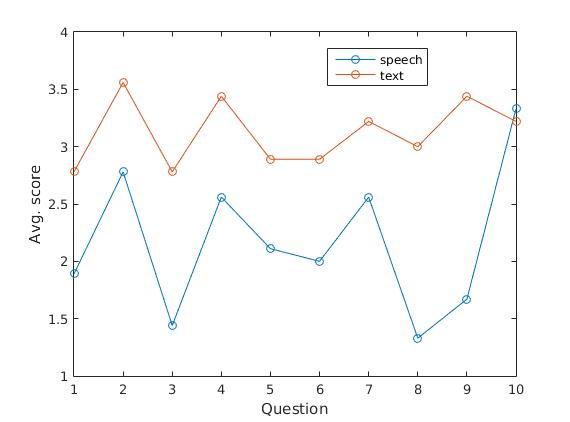
\includegraphics[width=0.8\textwidth]{images/sus.jpg}
  \caption{Bladiblala}\label{sus_table}
\end{figure}

\begin{table}[h!]
  \centering
  \begin{tabular}{ccc}
    \toprule
    Speech &   & Text\\
    \midrule
    54.17 &   & 78.06\\
    \bottomrule
  \end{tabular}
  \caption{Caption for the table.}\label{tot_score}
\end{table}

satisfaction